\newpage
\subsection{Textual; Fast Cards}
\texHeader
\hypertarget{fastCard tex}{}

\begin{itemize}
  
\item[$\blacktriangleright$] Create a new eclass in ``LearningBoxLanguage" named \texttt{FastCard} that extends \texttt{Card}. It doesn't need any new
attributes, so leave its declaration empty (Fig.~\ref{fig:fastClass}).

\begin{figure}[htp]
\begin{center}
  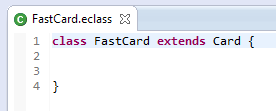
\includegraphics[width=0.45\textwidth]{eclipse_fastCardClass}
  \caption{A new Data Type}
  \label{fig:fastClass}
\end{center}
\end{figure}

\item[$\blacktriangleright$] Return to \texttt{Partition} to \texttt{check(card, guess)}, and edit the control flow by adding a second \texttt{if/else}
construct. Call the assertion pattern \texttt{isFastCard}, and the action pattern \texttt{promoteFastCard}. Keep the original \texttt{[promoteCard]} pattern in
the \texttt{else} statement.

\item[$\blacktriangleright$] Your workspace should now resemble Fig.~\ref{fig:isFastCard}.

\begin{figure}[htp]
\begin{center}
  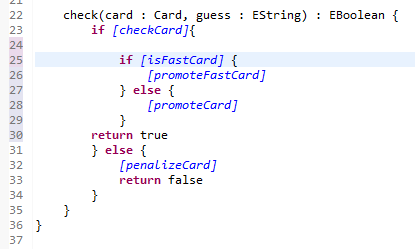
\includegraphics[width=0.7\textwidth]{eclipse_isFastCardFlow}
  \caption{Checking for \texttt{FastCard}}
  \label{fig:isFastCard}
\end{center}
\end{figure}

\item[$\blacktriangleright$] \texttt{isFastCard} is a simple, one line statement pattern. You need to create an assignment constraint to check a bounded object,
of type \texttt{FastCard}, against the type of card that was passed in through the parameter. Remember, to access paramter valuers, preface the name with a `\$'
symbol.

\item[$\blacktriangleright$] Your workspace should now resemble Fig.~\ref{fig:isFastCardPattern}.

\begin{figure}[htp]
\begin{center}
  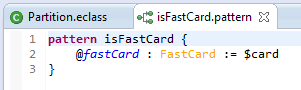
\includegraphics[width=0.5\textwidth]{eclipse_isFastCardPattern}
  \caption{A \texttt{FastCard} attribute constraint}
  \label{fig:isFastCardPattern}
\end{center}
\end{figure}

\item[$\blacktriangleright$] To establish \texttt{promoteFastCard.pattern}, first create the four main object variables - \texttt{@fastCard}, \texttt{@this},
\texttt{lastPartition}, and \texttt{box}. Immediately under \texttt{lastPartition}, also create a \texttt{next} NAC.

\vspace{0.5cm}

\item[$\blacktriangleright$] Your workspace should now resemble Fig.~\ref{fig:objVarFastCard}.

\begin{figure}[htp]
\begin{center}
  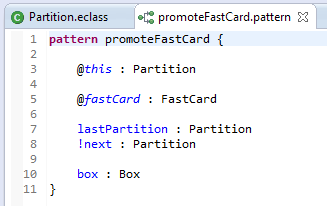
\includegraphics[width=0.6\textwidth]{eclipse_promoteFastCardObjVars}
  \caption{Object variables for \texttt{promoteFastCard}}
  \label{fig:objVarFastCard}
\end{center}
\end{figure}

\item[$\blacktriangleright$] When creating the necessary references, remember - this is the pattern that will be invoked when the fast card status has been
confirmed! This means that, in the appropriate variables, you'll want to:
(1) Link the partition to the current box.
(2) Remove \texttt{fastCard} from its current partition, and insert it into \texttt{lastPartition}
(3) Confirm \texttt{lastPartition} is in a box, then check to see if it has a \texttt{next} value.\footnote{If you need help remembering how NACs work, review
section 7}

\vspace{0.5cm}

\item[$\blacktriangleright$] Your final workspace should resemble Fig.~\ref{fig:promoFastCardFinal}

\newpage

\vspace*{1cm}

\begin{figure}[htp]
\begin{center}
  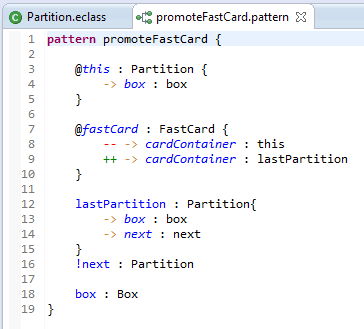
\includegraphics[width=0.6\textwidth]{eclipse_promoFastCardFinal}
  \caption{The completed fast card promotion pattern}
  \label{fig:promoFastCardFinal}
\end{center}
\end{figure}

\vspace{0.5cm}

\item[$\blacktriangleright$] You have now completed \texttt{every} method signature from your abstract syntax using SDMs - fantastic work! Build your project to
confirm there aren't any errors, and review Fig.~\ref{fig:sdm_fastcard_5} to see how \texttt{FastCard}s are implemented visually. We encourage you to read each
visual SDM section to understand the full scope of eMoflon's features, which start on page~\hyperlink{page.12}{12} but you are, of course, free to carry on.
  
\end{itemize}
